%
% File: chap01.tex
% Author: Victor F. Brena-Medina
% Description: Introduction chapter where the biology goes.
%
\let\textcircled=\pgftextcircled
\chapter{Introduction}
\label{chap:intro}

In the coming decade there is expected to be proliferation of new technologies that have been aided by recent developments in Artificial Intelligence(AI) and Machine Learning(ML). AI and ML have become topics of increasing interest in academic fields and industries globally. As a result, collaborations between these two fields has become increasingly common. 
With increase in computational power and the development of newer AI algorithms robotic technologies have greatly advanced and are now able to perform complex tasks that were once too difficult, dangerous or even impossible for humans to perform. Consequently, industries have benefited from the accuracy and efficiency provided by these robots. 

An area that has developed a wide range of interest currently is the topic of autonomous vehicles. The idea of autonomous vehicles is not new and as early as 2005, DARPA had invested heavily in the creation of unmanned trucks and organised for the Urban Challenge to allow for different teams to showcase their unmanned vehicles. However, due to the challenges such as low computational power and underdeveloped AI and ML systems, the resulting implementations were not practical and had a high fault rate of 1 fault in 100 miles compared to the human fault rate of around 1 in 100 million miles. Nonetheless, from this challenge, it was clear that the prospect of autonomous vehicles was plausible and indeed possible. 

\section{Why Autonomous Cars}

\subsection{Safety}
A major argument for self driving cars is the improved safety that they will provide on the road. According to a report released by the United States Department of Transport, National Highway Traffic Safety Administration(NHTSA), around 6,296,000 crashes occured in the year 2015 with 35,092 people losing their lives in these crashes. Of these crashes, around 94\% of them were as a result of human error. Worldwide, it is estimated that there were 1.2 million deaths in 2013 due to road crashes. 
In light of this, self driving cars could greatly reduce the number of road crashes. According to the Eno Centre of Transportation, if 90\% of the cars on the road were autonomous, there would be a reduction of 4,220,000 road crashes, this would save 21,700 lives. This is based on the fact that a large number of road crashes are a as a result of human error and therefore autonomous vehicles will be able to significantly reduce this number. 
However, this estimate is dependent on how well the AV system is designed to be able to handle complex, dynamic driving situations. 

\subsection{Environmental Impact}

According to the Environmental Protection Agency, more than a  quarter of greenhouse gases are from the transportation sector. A major contributor of this is traffic congestion due to various factors such as traffic destabilizing shockwave propagation and road accidents. Autonomous vehicles are able to mitigate this as they are able to gauge and calculate the motion vectors of different objects around them. By using traffic smoothing algorithms and smarter implementations such as the slot mechanism developed by MIT, traffic congestion can be greatly reduced and as a result lower fuel consumption. Furthermore, most companies working with AVs are moving towards electrical vehicles and thus reducing the impact of fossil fuels on the environment. 


This project seeks to develop further s



\section{Aims and Objectives}
The objectives of the  project are as follows:
\begin{enumerate}
	\item Detailed analysis of state-of-the-art Lidar-Based object detection deep neural networks.
	\item Implement voxel feature encoding layer for grouping point clouds
	\item Implement region proposal network for object detection from voxels.
	\item Test and evaluate the implemented neural network against results of state-of-the-art point cloud object detection methods.
\end{enumerate}

\section{Deliverables}

The deliverables are split into technical and analytical. 
\begin{itemize}
	 \item \textbf{End to end point cloud object detection RPN.} This will be a software implementation of the system that will be publicly available through a Github repository.
	\item \textbf{Evaluation report.} In this report, the following topics will be discussed. 
	\begin{enumerate}
		\item A review of related research and implementations tackling object detection using LiDAR cloud points. 
		\item Performance analysis of system and analysis criteria.
		\item A comparison between the implemented system and other state-of-the-art detection systems, potentially through a public benchmark. 
		\item The ethical and safety implications of the system and its viability in a real world setting. 
		\item Economic analysis of the LiDAR-based system and its potential impact on the development of AVs. 
		\item Validation of DNN performance with other public datasets containing data from AVs. 
	\end{enumerate}
\end{itemize}

\section{Added Value}

This project will implement and open source a sophisticated cloud point detection technique for use in autonomous vehicles.

In doing so, the project will democratize access to proprietary technology by Apple \cite{zhou2017voxelnet} to be used and developed further by future researchers working with object detection in point clouds.
Following the detailed review, I intend to propose ways through which this project can be implemented to reduce the cost of AVs in order to make them more viable. 
If successful, this project will provide a possible framework for the main stream adoption of AVs. 

\section{Research scope}
The focus of this project is mainly with regard to computer vision, deep learning and robotics. Computer vision is the task of obtaining, processing, analysing and contextualising visual information to produce numerical information that can be understood and manipulated by computers. This is necessary in order to process and analyse the LiDAR data. Deep learning is a broad term used to describe methods that utilise the use of deep neural networks that have a large number of layers. DNNs have become a heavily researched an invested area due to their ability to capture complex underlying models from data. This will be crucial for detecting objects from point clouds. 
This project will combine existing research using computer vision and deep learning such as \cite{qi2017pointnet}\cite{zhou2017voxelnet} to develop a Region Proposal Network capable of accurately detecting objects in point clouds. 

\section{Report structure}



\section{History and Current Setups}

In 2009, Google was the first major technology company to announce its self driving car project and within 18 months, it had developed a highly robust system that could handle some difficult roads. In the following years, there was an avalanche of companies that also announced their interest in developing self driving cars ranging from car manufacturers to other technology companies such as Apple, Samsung and NVIDIA.
Startups and other tertiary technology company began investing in developing systems that can be used in these autonomous vehicles. 

Currently, autonomous vehicles are grouped into 5 different categories by the NHTSA:
\begin{itemize}
    \item \textbf{Level 0} - No autonomy. 
    \item \textbf{Level 1} - Basic driver assistance built into vehicle design.
    \item \textbf{Level 2} - Partially autonomous but driver expected to monitor environment at all times.
    \item \textbf{Level 3} - Conditionally autonomous with the driver not required to monitor the environment but is required to take back control if need be.
    \item \textbf{Level 4} - Highly autonomous with the vehicle capable of handling most conditions but the driver has the option to take control. 
    \item \textbf{level 5} - Completely autonomous with the vehicle capable of handling all conditions.
\end{itemize}






\subsection{Componenents of a Self Driving Car}

Most self-driving cars consist of 4 main components: 
\begin{itemize}
    \item \textbf{LiDAR} - LiDAR provides highly detailed 3D information about the evnironment around the vehicle and objects in it. LiDAR operates by sending out pulses of lasers and recording the reflections of the pulses from objects. By comparing this with the time taken for the lasers to be reflected(time of flight) and their direction, the distance of these objects can be calculated and mapped in a point cloud. 
    \begin{equation*}
        distance = \frac{time \times \text{speed of light}}{2}
    \end{equation*}
    
    To achieve a high level of accuracy, the LiDAR has to send out a large enough number of lasers in different directions fast enough to create an accurate point cloud representation of the environment around it. As such, LiDAR systems have multiple channels(emitter/receiver pairs) angled vertically that  emit hundreds of thousands of lasers per second.
    
    \subsubsection{Cost}
    LiDAR systems require complex optical systems that are expensive to build. As such they are the most expensive sensor in AVs. Consequentially, the cost of production of LiDARs increase greatly as the number of channels increase. More channels allow for more accurate representations of the surrounding environment which is necesary for safer navigation of AVs, however this would not be economically feasible. 
    As such, different companies have developed different types of LiDAR in order to still produce accurate point clouds at a reasonable price. 

    \begin{itemize}
        \item \textbf{Mechanical Mirror}
        \item \textbf{Solid State}
        \item \textbf{Optical Phase Array}
        \item \textbf{Microelectromechanical systems (MEMS)}
        \item \textbf{3D Flash}
    \end{itemize}
    
   
    \item \textbf{Cameras} - Cameras mounted on the vehicle are used for classification and identification of various objects on the road. This is important for recognising traffic rules from traffic signs or road markings as well as determining the nature of objects on the road. 
    Cameras can also be used to create 3D maps of the surrounding environment.By combining two cameras, a stereo image can be captured that provides depth information. Alternatively, by combining a camera and IR Laser sensor for depth estimation, RGB-D images are obtained and mapped in a point cloud.

    \subsubsection{Cost}
    
    
    \item \textbf{Position Estimators} - Position estimators are a group of sensors used for navigation of the vehicle. These include GPS systems, odometers and gryometers. 
    \item \textbf{Distance Sensors} - Distance sensors such as radars and sonars are important for gauging the distance of objects on the road. 
    Radars are the most commonly used distance sensors and they work by transmitting radio waves and recording the reflected radio waves from objects. As compared to cameras and LiDARs, radars work well in a variety of low visibility scenarios such as poor weather. 
    However, the reflectivity of these radio waves depends on the nature of objects, their size, absorbtion characteristics and the transmitting power. As such, it is may not be effective for detecting objects with low absorbtion characteristics such as pedestrians and animals.
    
    \item \textbf{Processing Unit} - In order to process all the data from the sensors in the vehicle, AVs require powerful processing units in order to be able to process all this data in real time. Most of the ML/AI algorithms used for detecting and identifying objects from LiDAR and camera data demand large amounts of processing power. This is achieved through the use of CPUs, GPUs, FPGA or combinations with each other. 
    \subsubsection{Cost}
    Due to 
    
    
\end{itemize}


\begin{figure}[h]
    \centering
    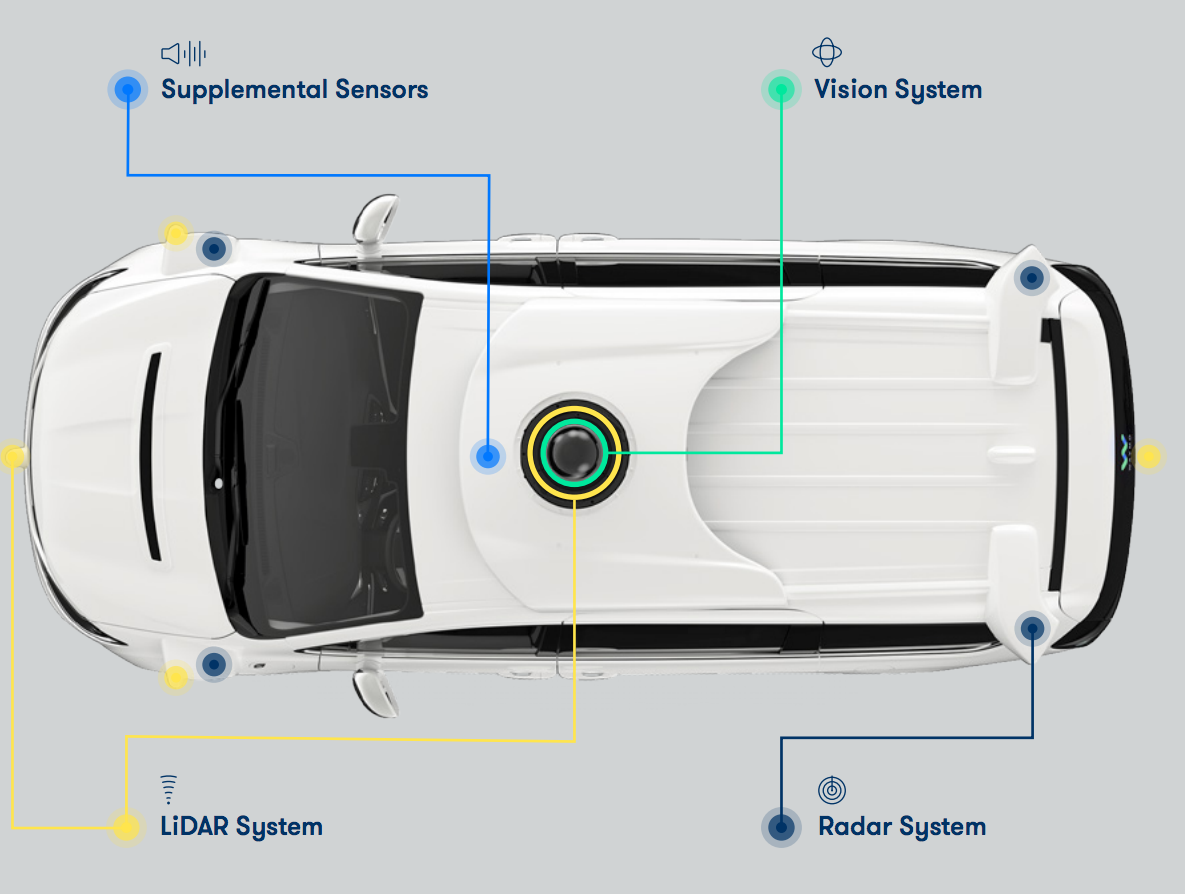
\includegraphics[width=\textwidth]{media/waymo.png}
    \caption{Components of Waymo's Self Driving Car (Waymo)}
    \label{fig:my_label}
\end{figure}

As seen from the table above, a wide range of sensors are used in AVs with each . This is essential for accurate navigation of the AV and therefore multiple sensors are fused together in order to provide enough data to achieve this. Given the large number of sensors, a major inhibiting factor in the production of AVs is the cost of sensors. Table \ref{cost} highlights the cost of the various sensors.




- Cost analysis 
- Attempts to minimise cost 
- Tradeoffs 
\section{Conclusion}

As highlighted from the previous section, each of the components serve a crucial purpose in AVs. It is evident that these components complement each other in order to adapt to their shortcomings.

From this a tradeoff between safety, cost, autonomy, power and viability cleary emerges with regard to producing autonomous vehicles. 
In this case, the following terms can be explained as below

\begin{itemize}
    \item \textbf{Safety}
    \item \textbf{Cost}
    \item \textbf{Autonomy}
    \item \textbf{Power}
    \item \textbf{Viability}
\end{itemize}


Cost increase viability decrease, safety increase, autonomy increase. power increase, vice versa is true 
Autonomy increase, cost increase, power increase, safety increase, viability decrease.
Power increase, viability decrease, cost increase










